\chapter{The scattering formula in the plane--plane geometry}
\label{chapter_scattering_pp}

In his original paper of 1984 \cite{Casimir1948}, Casimir considered two
parallel, perfectly conducting plates in vacuum at temperature $T=0$, and found
an attracting force due to vacuum fluctuations. Before we investigate the
Casimir effect in the plane--sphere configuration in the next chapter, we first
apply the scattering formula to the simpler plane--plane geometry. We will
rederive Casimir's famous formula, and also derive expressions for lossy Drude
metals at nonzero temperatures. We will introduce the scattering approach and
the results of this chapter will be used in chapter \ref{chapter_pfa} for the
description of the plane--sphere configuration in the proximity force
approximation (PFA).

We consider two parallel plates which are infinite in the $x$- and
$y$-directions and separated by a distance $d$. The lower plate is labeled as
plate 1, the upper plate is labeled as plate 2. We also assume that the plates
are thick enough to be considered as a bulk. This way, we may describe the
dielectric function by the Drude, plasma or perfect reflectors model, and the
reflection coefficients are given by the Fresnel coefficients.


\section{Round-trip operator}

\begin{figure}[t]
\begin{center}
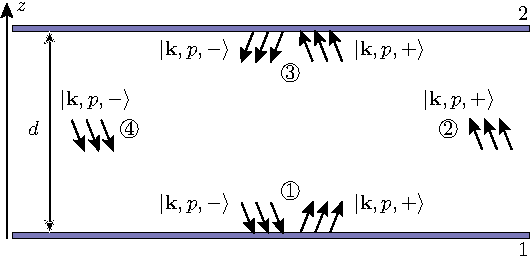
\includegraphics[scale=1.5]{images/roundtrip_pp.pdf}
\end{center}
\caption{The matrix $\mathcal{M}$ describes a round trip within the cavity:
\textcircled{1} Reflection on plane 1 yields the Fresnel coefficient $r_p$,
\textcircled{2} translation from plane 1 to plane 2 yields a phase factor $\e^{\imag k_z d}$,
\textcircled{3} reflection on plane 2 yields another Fresnel coeffient $r_p$, and
\textcircled{4} translation back to plane 1 yields a second phase factor $\e^{\imag k_z d}$.}
\label{fig:scattering_pp_roundtrip}
\end{figure}

The scattering approach is described in many publications with different
focus on geometry, finite conductivity and temperature \cite{Durand, PhysRevLett.102.230404, ThermalCasimirEffect, ScatteringApproach,
CasimirWithinScatteringTheory, Lambrecht:CasimirScatteringApproach,
ScatterinTheoryApproach, Reynaud:ScatteringApproach}.
The Casimir free energy is given as a sum over the Matsubara frequencies
$\omega_n$
\begin{equation}
\F = \kb T {\sum_{n=0}^\infty}^\prime \log\det \mathcal{D}(\omega_n), \\ \omega_n = \frac{2\pi n \kb T}{\hbar},
\end{equation}
where $\mathcal{D}$ is the scattering operator and the primed sum indicates
that the $n=0$ term is weighted by $1/2$.
The configuration is time-invariant, thus
the frequency $\omega$ is preserved during scattering processes and the
scattering operator is block diagonal with respect to $\omega$.
The scattering operator is related to the round-trip operator $\mathcal{M}$ by
\begin{equation}
\mathcal{D}(\omega) = \Id-\mathcal{M}(\omega).
\end{equation}
The round-trip operator $\mathcal{M}$ consists of the reflection operator at
plane 1, the translation operator from plane 1 to plane 2, the reflection operator
at plane 2, and the translation operator from plane 2 to plane~1
\begin{equation}
\mathcal{M} = \mathcal{T}_{1\leftarrow 2} \mathcal{R}_2 \mathcal{T}_{2\leftarrow 1} \mathcal{R}_1.
\end{equation}
The operator $\mathcal{M}$ thus corresponds to one round trip within the
cavity. The scattering operator $\mathcal{D}$ may be interpreted as the
difference between doing a round trip and not doing a round trip \cite{Durand}.
The reader might note that the round-trip operator is only unique up to cyclic
permutations. However, it follows from \textsc{Sylvester}'s determinant theorem 
\begin{equation}
\det\left(\mathbbm{1} - AB\right) = \det\left(\mathbbm{1} - BA\right)
\end{equation}
that the free energy $\F$ is invariant under permutations.

The translation and reflection operators of the plates are diagonal in the
plane wave basis, because its basis functions are eigenfunctions of the
momentum operator. The reflection of plane waves at a plane preserves the
transverse wave vector and polarization, but changes the direction of
propagation:
\begin{align}
\mathcal{R}_1 \ket{\, \vec k, p, +} &= 0                                          & \mathcal{R}_2 \ket{\, \vec k, p, +} &= r_p^{(2)}(\omega, k) \ket{\, \vec k, p, -} \\
\mathcal{R}_1 \ket{\, \vec k, p, -} &= r_p^{(1)}(\omega, k) \ket{\, \vec k, p, +} & \mathcal{R}_2 \ket{\, \vec k, p, -} &= 0
\end{align}
The coefficients are given by the Fresnel coefficients $r_p(\omega,k)$. For the
sake of simplicity, we assume that both plates have identical optical
properties and set $r_p\equiv r_p^{(1)} = r_p^{(2)}$, a generalization to
different Fresnel coefficients is trivial. The translation operators are also
diagonal in the plane wave basis
\begin{equation}
\mathcal{T}_{2\leftarrow1} \ket{\, \vec k, p, \phi} = \e^{\imag \phi k_z d} \ket{\, \vec k, p, \phi}, \\ \mathcal{T}_{1\leftarrow2} \ket{\, \vec k, p, \phi} = \e^{-\imag \phi k_z d} \ket{\, \vec k, p, \phi},
\end{equation}
and yield a phase factor dependent on the direction of propagation.

We now derive the matrix elements of $\mathcal{M}$ in the
plane wave basis. The round-trip operator acting on a plane wave propagating in
upward direction yields
\begin{equation}
\mathcal{M} \ket{ \, \vec k, p, +} = \mathcal{T}_{1\leftarrow 2} \mathcal{R}_2 \mathcal{T}_{2\leftarrow 1} \mathcal{R}_1\ket{ \, \vec k, p, +} = 0.
\end{equation}
For a plane wave propagating in downward direction, we find
\begin{equation}
\mathcal{M} \ket{ \, \vec k, p, -} = \mathcal{T}_{1\leftarrow 2} \mathcal{R}_2 \mathcal{T}_{2\leftarrow 1} \mathcal{R}_1\ket{ \, \vec k, p, -} = r_p^2(\omega,k) \, \e^{2 \imag k_z d} \, \ket{\, \vec k, p, -}.
\end{equation}
We see that the round-trip operator is diagonal in the plane wave
basis. The transverse wave vector and the polarization remain spectators within
a round trip. The round trip is illustrated in Fig.
\ref{fig:scattering_pp_roundtrip}.

\section{Free energy}
\label{section_scattering_pp_free_energy}

As the round-trip operator is diagonal in the plane wave basis, the determinant
is given by the product of the diagonal matrix elements. Thus the product is given
as a sum
\begin{equation}
\log \det \mathcal{D}(\omega) = \log \prod_{\vec k, p} \left(1 - r_p^2 \e^{2 \imag k_z d}\right) = \sum_{\vec k, p} \log{\left(1 - r_p^2 \e^{2 \imag k_z d}\right)}
\end{equation}
over the polarizations $p=\TE,\TM$ and the wave vectors
\begin{equation}
\label{eq:scattering_pp_wavevector}
k_{x,y} = \frac{2\pi n_{x,y}}{L_{x,y}}, \\ n_{x,y}\in \mathbb{Z}.
\end{equation}
Eq. \eqref{eq:scattering_pp_wavevector} can be deduced using box quantization,
$L_x$, $L_y$ correspond to the lengths of the plates in $x$- and $y$-direction.
When the area $A \equiv L_xL_y$ of the plates tends to infinity, the summation
over the wave vectors becomes dense and we can replace the sum by an integral
\cite{ThermodynamicalLimit}
\begin{equation}
\sum_{\vec k} \rightarrow \frac{A}{(2\pi)^2} \int \mathrm{d}^2 \vec k = \frac{A}{(2\pi)^2} \int_0^\infty \mathrm{d}k \, k \int_0^{2\pi} \mathrm{d}\varphi_k = \frac{A}{2\pi} \int_0^\infty \mathrm{d}k \, k.
\end{equation}
%\begin{align}
%\nonumber
%\log \det \mathcal{D}(\omega) &= A \sum_{p=\TE,\TM} \int \frac{\mathrm{d}^2 \vec k}{(2\pi)^2} \log{\left(1-\rho_p\right)} \\
%&= \frac{A}{4\pi^2} \int_0^\infty \mathrm{d}k \, k \int_0^{2\pi} \mathrm{d}\varphi_k \, \log{\left[\left(1-\rho_\TE\right) \left(1-\rho_\TM\right)\right]} \\
%&= \frac{A}{2\pi} \int_0^\infty \mathrm{d}k \, k \log{\left[\left(1-\rho_\TE\right) \left(1-\rho_\TM\right)\right]}
%\end{align}
The Fresnel coefficients and the phase factor depend on $k$ only and therefore
the integration over $\varphi_k$ yields $2\pi$. The logarithm of the
determinant of the scattering operator simplifies to an integration over $k$
\begin{equation}
\label{eq:scattering_pp_integral_plain}
\log \det \mathcal{D}(\omega) = \frac{A}{2\pi} \int_0^\infty \mathrm{d}k \, k \, \log{\left[\left(1-r_\TE^2\e^{2\imag k_z d}\right) \left(1-r_\TM^2 \e^{2\imag k_z d}\right)\right]}.
\end{equation}
The integral \eqref{eq:scattering_pp_integral_plain} is an oscillatory integral
and hard to evaluate numerically. As the integrand is analytic in the upper
complex half-space \cite{LossyOpticalCavities}, we can change the axis of
integration according to \textsc{Cauchy}'s integral theorem to imaginary
frequencies $\omega = \imag \xi$, $\xi \in \mathbb{R}$. We will use the
definitions $k_z \equiv \imag\kappa$ and $\kappa \equiv \sqrt{\xi^2/\c^2+k^2}$
that we have introduced in section \ref{section_optical_properties_fresnel}.
The Wick rotation changes 
$\omega \to \imag \xi$ and $k_z \to \imag\kappa$
in \eqref{eq:scattering_pp_integral_plain}. After the Wick rotation, the free energy
at finite temperature can be written as
\begin{equation}
\label{eq:scattering_pp_int}
\frac{\mathcal{F}}{A} = \frac{\kb T}{2\pi} {\sum_{n=0}^\infty}^\prime \int_{\xi_n/\c}^\infty \mathrm{d}\kappa \, \kappa \, \log{\left[\left(1-\rho_\TE\right)\left(1-\rho_\TM\right)\right]}, \\ \rho_p(\xi,\kappa) = r_p^2(\imag\xi_n,\kappa) \, \e^{-2\kappa d}.
\end{equation}
The integrand is now damped by an exponential factor which ensures fast
convergence of the integral. The Fresnel coefficient $r_p$
depends on the dielectric function $\epsilon(\imag\xi)$ of the metal.
Eq. \eqref{eq:scattering_pp_int} has a wide range of validity: We have
made no assumptions on the reflection coefficients $r_p$. The dielectric
function may be given by the Drude or plasma model, the model of perfect
reflectors or from experimental data.
We will consider Drude and perfect mirrors in the following sections.


\section{Perfect reflectors}

\begin{figure}
\begin{minipage}[b]{.5\linewidth}
\centering
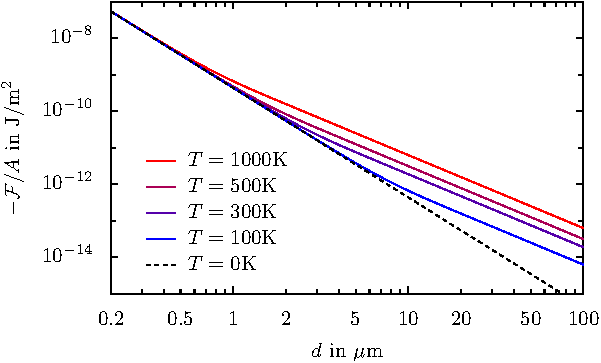
\includegraphics[scale=0.76]{plots/pp/pp_perf.pdf}
\subcaption{perfect reflectors}
\end{minipage}%
\begin{minipage}[b]{.5\linewidth}
\centering
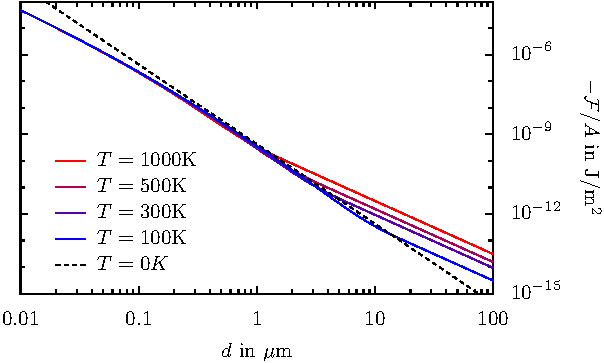
\includegraphics[scale=0.76]{plots/pp/pp_gold.pdf}
\subcaption{Drude model}
\end{minipage}
\caption{The Casimir free energy for different temperatures for a) perfect
reflectors and b) Drude metals. The values of the parameters for the Drude
model are $\omega_\text{P}=1.385\cdot10^{16}\mathrm{s}^{-1}$,
$\gamma=5.54\cdot10^{13}\mathrm{s}^{-1}$ and correspond to gold. The dashed
lines correspond to $T=0$ for perfect reflectors in both plots.}
\label{fig:scattering_pp_perf_gold}
\end{figure}


For perfect reflectors integral \eqref{eq:scattering_pp_int} can be
computed analytically. The Fresnel coefficients for perfect reflectors are
given by $r_\TM=-r_\TE=1$. After substituting $t=2\kappa d$ the free energy
becomes
\begin{equation}
\frac{\mathcal{F}^\text{perf}}{A} = \frac{\kb T}{4\pi d^2} \sum_n^\prime \int_{2\xi_n d/\c}^\infty \mathrm{d}t \, t \, \log{\left(1-\e^{-t}\right)}
\end{equation}
and the integral can be evaluated in terms of the polylogarithms $\text{Li}_2$ and $\text{Li}_3$
\begin{equation}
\label{eq:scattering_pp_F_perfect}
\frac{\mathcal{F}^\text{perf}}{A} = -\frac{\kb T}{4\pi d^2} \sum_n^\prime \left[ \text{Li}_3\left(\e^{-2\xi_n d/\c}\right) + \frac{2\xi_n d}{\c} \text{Li}_2\left(\e^{-2\xi_n d/\c}\right)\right].
\end{equation}
A short description about basic properties of polylogarithms can be found in
appendix \ref{appendix_polylog}. As the Matsubara frequency is proportional to
$nT$, the argument of the polylogarithms becomes small for high temperatures.
For small arguments the polylogarithms may be approximated by $\text{Li}_s(x)
\simeq x$. In the high temperature limit contributions to the free energy
become negligible for $n>0$ and we find
\begin{equation}
\label{eq:scattering_pp_F_perfect_hiT}
\frac{\mathcal{F}^\text{perf}_\text{HT}}{A} = -\frac{\kb T \zeta(3)}{8\pi d^2} \\ \text{for} \sep \lambda_T \ll 2\pi d,
\end{equation}
where $\zeta$ is the Riemann zeta function,
$\zeta(3)=\text{Li}_3(1)\approx1.20206$, and $\lambda_T = \hbar\c/(\kb T)$ is
the thermal wavelength. For temperature $T=0$ the sum becomes dense and we can
replace it by an integral
\begin{equation}
\kb T \sum_n^\prime \to \hbar \int_0^\infty \frac{\mathrm{d}\xi}{2\pi}.
\end{equation}
This integral can be evaluated analytically and we find Casimir's famous
formula
\begin{equation}
\label{eq:scattering_pp_F_perfect_T0}
\frac{\mathcal{F}^\text{perf}_{T=0}}{A} = - \frac{\pi^2 \hbar \c}{720 d^3}.
\end{equation}
This expression is remarkable as it only depends on fundamental constants like
the Planck constant $\hbar$, the speed of light $\c$, and the separation $d$ of
the plates. In particular, this result seems to be independent of the fine
structure constant $\alpha$. However, this is just an artefact of the idealized
description of the metals as perfect reflectors \cite{jaffe2005casimir}.

In Fig. \ref{fig:scattering_pp_perf_gold} a) the Casimir free energy for
perfect reflectors as a function of the separation $d$ is plotted for different
temperatures. The dashed line corresponds to the zero temperature limit. For
small separations the free energy coincides with the zero temperature limit.


\section{Drude mirrors}
\label{section_scattering_pp_drude}

Real metals show a more complicated behaviour. The qualitative effect may be
understood by a simple argument: Due to finite conductivity, electromagnetic
waves are able to penetrate the metal. This effect is known as skin effect and
the penetration depth $\delta$ is called skin depth. The skin depth increases
the effective distance between the two plates to $d_\text{eff}\approx
d+2\delta$. Thus we expect the absolute value of the Casimir free energy to be
smaller for Drude metals than for perfect mirrors. Small separations of the
plates correspond to high temperatures and thus high frequencies at which the
mirrors become transparent. The penetration depth becomes large and the free
energy deviates from the result for perfect mirrors \cite{jaffe2005casimir}.

For high temperatures it is sufficient to consider only the $n=0$ term. In this
case the Matsubara frequency is $\xi_0=0$ and the Fresnel coefficients become
$r_\TE=0$ and $r_\TM=1$. Then \eqref{eq:scattering_pp_int} can be solved
analytically and we obtain
\begin{equation}
\frac{\mathcal{F}^\text{Drude}_\text{HT}}{A} = -\frac{\kb T \zeta(3)}{16 \pi d^2},
\end{equation}
which differs by a factor $2$ from the result for perfect reflectors. This is a
consequence of the different behaviour of the Fresnel coefficient for the TE
mode: For Drude mirrors the reflection coefficient is $r_\TE = 0$, while it is
$r_\TE = -1$ for perfect mirrors.

Fig. \ref{fig:scattering_pp_perf_gold} b) shows the free energy for Drude
mirrors as a function of the separation $d$ for different temperatures. The
dashed line corresponds to the zero temperature limit for perfect reflectors.
For small separations the free energy differs from the zero temperature limit
for perfect reflectors because of plasma oscillations.


\section{Entropy}

The Casimir entropy can be derived from the free energy by
\begin{equation}
S = -\frac{\partial \mathcal{F}}{\partial T}.
\end{equation}
While the entropy is non-negative for perfect reflectors, we find negative
values of the entropy in the Drude model over a wide separation distance range
and for not too high temperatures. Fig. \ref{fig:scattering_pp_entropy} shows
negative entropies as a function of temperature and separation in the Drude
model. We will delay the discussion of the physical implications of negative
entropies and come back to this question in chapter
\ref{chapter_negative_entropies}. At this point, we just notice that the
Casimir entropy may become negative in the plane--plane geometry for Drude
mirrors.

\begin{figure}
\begin{center}
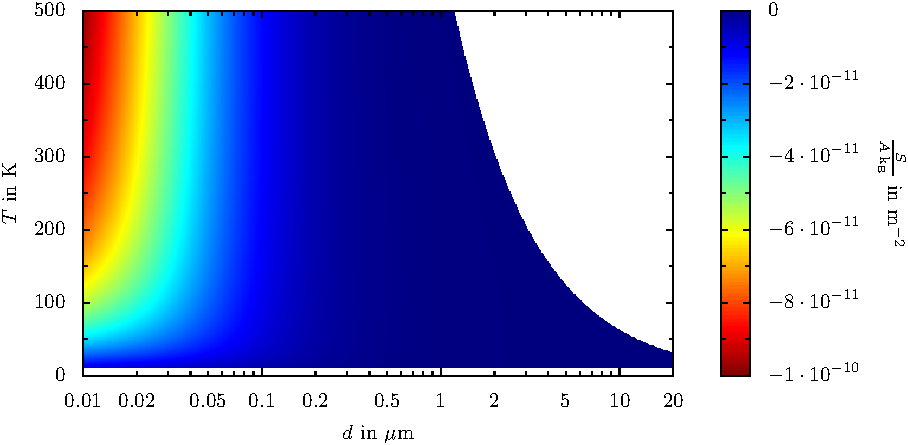
\includegraphics[scale=1]{plots/pp/entropy/plot.pdf}
\end{center}
\caption{Negative Casimir entropy dependent on temperature $T$ and separation
$d$ in the Drude model in the range $11\mathrm{K} \le T \le 499\mathrm{K}$ and
$0.01\mu\mathrm{m} \le d \le 20\mu\mathrm{m}$. White areas in this range
correspond to positive entropies. While we find parameters for which the
entropy is negative, the third law of thermodynamics is not violated as
$S(T\to0)\to0$. The material parameters in this plot are those of gold:
$\omega_\text{P}=1.385\cdot10^{16} \, \mathrm{s}^{-1}$,
$\gamma=5.54\cdot10^{13} \, \mathrm{s}^{-1}$}
\label{fig:scattering_pp_entropy}
\end{figure}
